\section{\uppercase{Theoretical Background}}
\label{sec:theoretical}

This section presents the proposed \textbf{RALA-ChangeFormer}, a computationally efficient variant of ChangeFormer in which the quadratic Multi-Head Self-Attention (MHSA) is replaced with rank-augmented linear attention (RALA). In order to provide a better understanding, we organized the paragraphs: (i) a brief overview of ChangeFormer, (ii) a clear formulation of Rank-Augmented Linear Attention (RALA), and (iii) the integration into the bi-temporal encoder–decoder design. In addition, this section introduces the theoretical formulation that underpins the proposed method, providing the mathematical foundations required for its implementation and analysis.

\subsection{ChangeFormer}
\label{subsec:cf_overview}

ChangeFormer~\cite{Bandara2022ChangeFormer} is a hierarchical Siamese encoder-decoder architecture designed for bi-temporal building change detection. An overview of the full architecture is shown in Fig.~\ref{fig:changeformer_architecture}. Given two VHR images 
$I_{t_1}$ and $I_{t_2}$, the model processes them through a shared convolutional encoder to obtain multi-scale feature maps
\begin{equation}
F_{t_1}^{(l)},\, F_{t_2}^{(l)} \in \mathbb{R}^{H_l \times W_l \times C_l},
\end{equation}
where $l$ denotes the resolution level in the hierarchy. The encoder follows the same design principle as hierarchical Vision Transformer backbones such as Swin~\cite{Teng2023SwinCD}: the spatial resolution is progressively reduced while channel dimensionality increases, enabling the model to capture both fine-grained local texture and broader semantic context across scales.

At each scale, the bi-temporal feature maps are concatenated channel-wise and projected into a sequence of tokens via a lightweight patch embedding module:
\begin{equation}
X^{(l)} = \mathrm{PatchEmbed}\!\left(F_{t_1}^{(l)} \,\Vert\, F_{t_2}^{(l)}\right)
      \in \mathbb{R}^{N_l \times C_l},
\end{equation}
where $N_l = H_lW_l$ is the number of tokens at level $l$.

The decoder is composed of a cascade of Transformer blocks operating at multiple resolutions. Each block contains Multi-Head Self-Attention (MHSA) and a feed-forward network (FFN), refining token representations through long-range spatio-temporal interactions before upsampling and fusion into the final change mask.

Because MHSA has quadratic complexity in the sequence length ($\mathcal{O}(N_l^2)$), the decoder becomes the dominant computational bottleneck for VHR imagery where $N_l$ is large. Furthermore, this architecture does not incorporate the shifted-window mechanism used in Swin Transformer~\cite{Teng2023SwinCD}, which further limits its ability to efficiently capture long-range dependencies at lower computational cost. This motivates the integration of a more efficient attention mechanism—specifically, rank-augmented linear attention—to reduce computational cost while preserving the representational capacity required for accurate change detection.


\subsection{Rank-Augmented Linear Attention}
\label{subsec:rala}

Linear attention methods aim to reduce the $\mathcal{O}(N^2)$ cost of standard softmax attention by replacing the kernel with a feature map $\kappa(\cdot)$. Standard attention is defined as
\begin{equation}
\mathrm{Attn}(Q,K,V)=\mathrm{softmax}\!\left(\frac{QK^\top}{\sqrt{d}}\right)V,
\label{eq:softmax_attention}
\end{equation}
where $Q,K,V\in\mathbb{R}^{N\times d}$ \cite{Vaswani2017Attention} contain the queries, keys, and values for the $N$ input tokens (each row $Q_i$ is the query vector of token $i$), and $d$ denotes the hidden embedding dimension. Forming the dense matrix $QK^\top$ produces quadratic time and memory cost.

Linear attention replaces the softmax kernel with a feature map:
\begin{equation}
\mathrm{Attn}_{\text{lin}}(Q,K,V)=\kappa(Q)\big(\kappa(K)^\top V\big),
\label{eq:linear_attention}
\end{equation}
where $\mathcal{\kappa(.)}$ is a kernel feature map, reducing the complexity to $\mathcal{O}(Nd)$.  
The intermediate matrix
\begin{equation}
\kappa(K)^\top V \in\mathbb{R}^{d\times d}
\label{eq:B_def}
\end{equation}
acts as a global key–value aggregation buffer. In practice, the equation \ref{eq:B_def} often becomes \emph{low-rank} because many key vectors are nearly collinear. This collapse in feature diversity limits representational power and degrades dense prediction performance.

\paragraph{Rank Augmentation.}
RALA~\cite{Fan2025RALA} addresses this by explicitly increasing the rank of $B$. Let $K_j$ and $V_j$ denote the key and value vectors of token $j$. RALA constructs
\begin{equation}
B=\sum_{j=1}^{N}\alpha_j\,\kappa(K_j)^\top V_j ,
\label{eq:rala_rank_aug}
\end{equation}

\begin{equation}
N=\sum_{j=1}^{N}\alpha_j
\label{eq:rala_alpha_aug}
\end{equation}

\noindent where $\alpha_j$ reweights each token using a \emph{global query vector}
\begin{equation}
Q_{\mathrm{g}}=\frac{1}{N}\sum_{i=1}^N Q_i,
\label{eq:global_query}
\end{equation}
encoding the overall semantic content of the sequence. The weights are computed as
\begin{equation}
\alpha_j=N \times \frac{\exp(Q_{\mathrm{g}}\kappa(K_j)^\top)}
{\sum_{m=1}^{N}\exp(Q_{\mathrm{g}}\kappa(K_m)^\top)},
\label{eq:alpha_softmax}
\end{equation}
which emphasizes information-rich tokens and increases the effective rank of $B$.

\paragraph{Output Feature Modulation.}
Even if $B$ achieves a full-rank state, the output features
\begin{equation}
Y_i=\kappa(Q_i)\,B
\label{eq:Y_pre_modulation}
\end{equation}
may still be low-rank.  
This follows from the matrix inequality
\begin{equation}
\mathrm{Rank}(Y)\le \min\big(\mathrm{Rank}(\kappa(Q)),\,\mathrm{Rank}(B)\big)\le d,
\label{eq:rank_inequality}
\end{equation}
which states that the output cannot have rank greater than its limiting factors: the diversity of queries \(\kappa(Q)\) and the diversity of the aggregated buffer \(B\). When $\kappa$ contains many correlated query vectors (common in remote sensing patches), $\mathrm{Rank}(\kappa(Q))<d$, causing information loss even if $B$ is full-rank.

To restore feature diversity, RALA introduces a token-wise modulation step:
\begin{equation}
Y_i=\phi(X_i)\odot \Big(\kappa(Q_i)\,B\Big),
\label{eq:Yi_modulated}
\end{equation}
where $\phi(\cdot)$ is a token-dependent transform applied only for modulation, and $\odot$ denotes the Hadamard product.  
This injects token-specific information without increasing the asymptotic cost and increases the expressive rank of the output.
This operation injects token-specific information into the output features, complementing the global mixing performed by $B$ and effectively increasing the expressive rank of $Y$. The modulation is applied only channel-wise, preserving the linear-time complexity of the attention operation.

\begin{figure}[t]
    \centering
    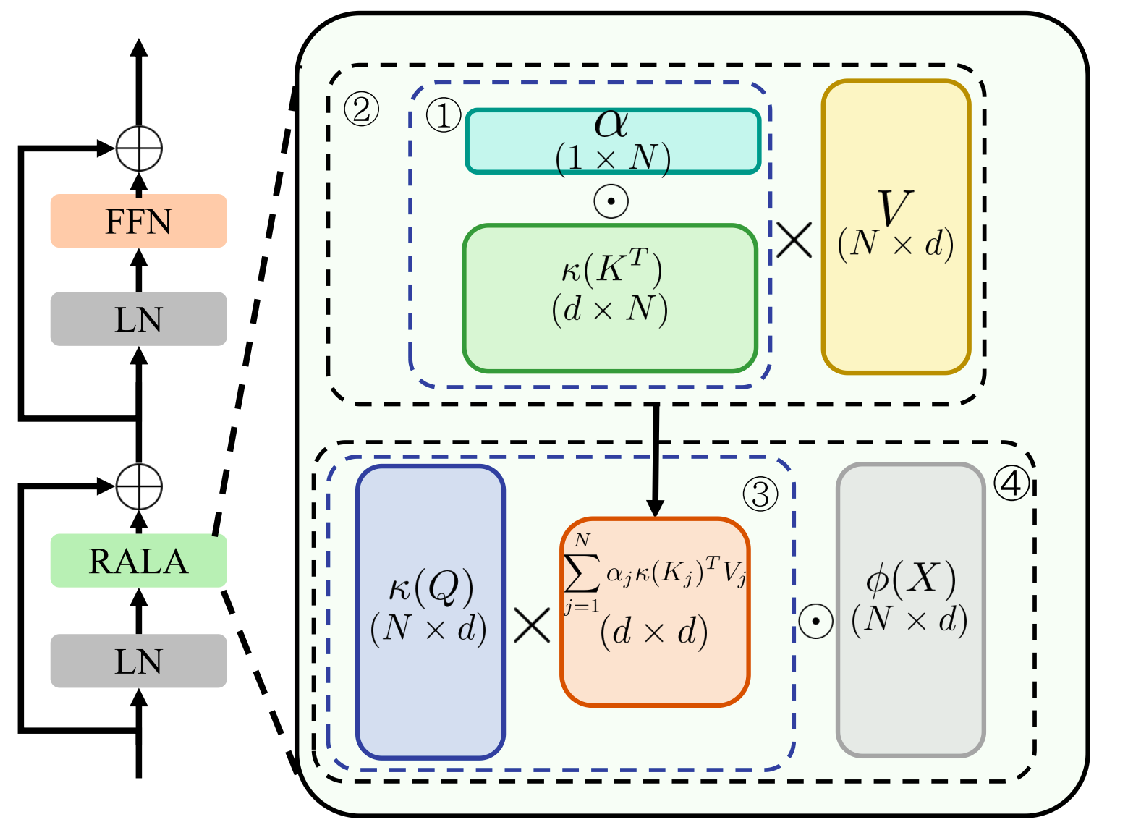
\includegraphics[width=\linewidth]{images/RALA.png}
    \caption{RALA Transformer block replacing the standard MHSA module. Recovery from RALA original paper \cite{Fan2025RALA}}
    \label{fig:rala_block}
\end{figure}